%!TeX TS-program = latexmk --pdf  -pdflatex=lualatex 
%!TeX encoding = UTF-8 Unicode 
%!TeX spellcheck = en-US
% !BIB TS-program = biber
%%%%%%%%%%%%%%%%%%%%%%%%%%%%%%%%%%%%%%%%%%%%%%%%%%%%%%%%%%%%%%%%%%%%%
%!TeX TS-program = Lualatex 
%!TeX encoding = UTF-8 Unicode 
%!TeX spellcheck = en-US
%!TEX root = PerrinetBednar15srep.tex
%%%%%%%%%%%%%%%%%%%%%%%%%%%%%%%%%%%%%%%%%%%%%%%%%%%%%%%%%%%%%%%%%%%%%
\newcommand{\AuthorA}{Laurent U.~Perrinet}%
\newcommand{\AuthorB}{James A.~Bednar} %
\newcommand{\AddressA}{Institut de Neurosciences de la Timone \\
CNRS / Aix-Marseille Universit\'e}% - Marseille, France
\newcommand{\LongAddressA}{
Institut de Neurosciences de la Timone (UMR 7289),
Aix Marseille Universit\'e, CNRS \\
%Facult\'e de M\'edecine - B\^atiment Neurosciences,
27, Bd Jean Moulin,
13385 Marseille Cedex 05,
France}
\newcommand{\PhoneA}{+33.491 324 044}%
\newcommand{\AddressB}{Institute for Adaptive and Neural Computation\\
University of Edinburgh}%
\newcommand{\Website}{http://invibe.net/LaurentPerrinet}%
\newcommand{\Email}{Laurent.Perrinet@univ-amu.fr}%
\newcommand{\Title}{Edge co-occurrences can account for rapid categorization of natural versus animal images}% 88 chars <90
\newcommand{\ShortTitle}{Edge co-occurrences categorize natural images}%
\newcommand{\Abstract}{
Making a judgment about the semantic category of a visual scene, such as whether it contains an animal, is typically assumed to involve high-level associative brain areas. Previous explanations require progressively analyzing the scene hierarchically at increasing levels of abstraction, from edge extraction to mid-level object recognition and then object categorization. Here we show that the statistics of edge co-occurrences alone are sufficient to perform a rough yet robust (translation, scale, and rotation invariant) scene categorization. We first extracted the edges from images using a scale-space analysis coupled with a sparse coding algorithm. We then computed the ``association field'' for different categories (natural, man-made, or containing an animal) by computing the statistics of edge co-occurrences. These differed strongly, with animal images having more curved configurations. We show that this geometry alone is sufficient for categorization, and that the pattern of errors made by humans is consistent with this procedure. Because these statistics could be measured as early as the primary visual cortex, the results challenge widely held assumptions about the flow of computations in the visual system. The results also suggest new algorithms for image classification and signal processing that exploit correlations between low-level structure and the underlying semantic category.
}%
\newcommand{\Keywords}{natural scene statistics; edge co-occurrence; good continuation; association field; lateral connections}%
\newcommand{\Acknowledgments}{%
We are very grateful for the reviewers' and editor effort and time to improve this paper. 
L.U.P.\ was supported by EC IP project FP7-269921, ``BrainScaleS'' and 
ANR project "BalaV1" N°ANR-13-BSV4-0014-02. 
Thanks to David Fitzpatrick for allowing J.A.B.\ access to the laboratory 
in which the man-made images were taken. 
Correspondence and requests for materials 
should be addressed to LUP (email:\Email\ )%
\footnote{Code and supplementary material available 
at \url{\Website/Publications/PerrinetBednar15}.}. %
}%
\newcommand{\SignificanceStatement}{%
 Humans can very rapidly judge the category of an image, such as
 whether it contains an animal. Previous theories for this capability
 require hierarchical grouping of low-level edge elements into
 increasingly complex object representations. Here we show that the
 edges alone are sufficient for this judgment, if the patterns of
 co-occurrence between them are taken into account. For instance,
 images with animals tend to have contours that are more highly
 curved. These results suggest that humans could be using low-level
 statistical regularities to drive rapid but accurate high-level
 judgments, and could help improve computer vision systems.
 %% 100 words
}
\newcommand{\Highlights}{%
\begin{itemize}
\item Humans very efficiently judge the category of an image. 
 
\item Previous theories require hierarchical grouping of object representations. 
 
 \item We show that the edges alone are sufficient for this judgment.
 
 \item The pattern of edge co-occurrence is sufficient to categorize an image with an animal. 
 
 \item Humans could be using such low-level statistical regularities to drive decisions.

 \item Future computer vision systems could use such features.

\end{itemize}
}%
%%%%%%%%%%%%%%%%%%%%%%%%%%%%%%%%%%%%%%%%%%
%%%%%%%%%%%%%%%%%%%%%%%%%%%%%%%%%%%%%%%%%%
%%%%%%%%%%%%%%%%%%%%%%%%%%%%%%%%%%%%%%%%%%
%%%%%%%%%%%%%%%%%%%%%%%%%%%%%%%%%%%%%%%%%%
%%%%%%%%%%%%%%%%%%%%%%%%%%%%%%%%%%%%%%%%%%
\documentclass[a4paper]{article}
%% ========  polices de caracteres =============
\usepackage[T1]{fontenc}% 
\usepackage{lmodern}%
\usepackage{t1enc}
\usepackage{times}
%============ graphics ===================
\usepackage[pdftex]{graphicx}% 
\DeclareGraphicsExtensions{.pdf,.png}%
\graphicspath{{../figures/},{./}}% 

\usepackage[natbib=true,
			style=nature, %numeric-comp,
      		sortcites=true,
			abbreviate=true,
			maxcitenames=2,
			maxnames = 5,
%			firstinits=true,
%			uniquename=init,
%			sorting=none,
			doi=false,
			url=false,
			isbn=false,
			eprint=false,
			%texencoding=utf8,
			%bibencoding=latin1,
			%autocite=superscript,
%			backend=bibtex,
			%articletitle=false,
			]{biblatex}%
\AtEveryBibitem{
  \clearfield{month}
  \clearfield{day}
  \clearfield{note}
  \clearfield{comment}
%  \clearfield{edition}
%  \clearfield{publisher}
}
\addbibresource{../bib/PerrinetBednar15.bib}%
\DeclareFieldFormat{labelnumber}{\decrease{#1}}

\newcounter{num}
\newcommand{\decrease}[1]{\setcounter{num}{#1}\addtocounter{num}{20}\thenum}
%%%%%%%%%%%%%%%%%%%%%%%%%%%%%%
%% OPTIONAL MACRO FILES
\usepackage{tikz,tkz-euclide} \usetkzobj{all} % loading all objects
\usetikzlibrary{positioning} \usetikzlibrary{calc}
%%%%%%%%%%%%%%%%%%%%%%%%%%%%%%
\usepackage{sfmath}
%% The AMS math files are commonly used to gain access to useful features
%% like extended math fonts and math commands.
%\usepackage{amssymb,amsfonts,amsmath}
%%%%%%%%%%%%%%%%%%%%%%%%%%%%%%
\usepackage{float}
%============ hyperref ===================
\usepackage[unicode, linkcolor=blue, citecolor=blue, filecolor=black, urlcolor=blue, hidelinks]{hyperref}%
\hypersetup{%
pdftitle={\Title - Supplementary Material},%
pdfauthor={\AuthorA < \Email > \AddressA - \Website},%
pdfkeywords={\Keywords},%
%pdfsubject={\Acknowledgments}%
}%
%%%%%%%%%%%% authblk %%%%%%%%%%%%%%%
\usepackage{authblk}%
\title{Supplementary Information to \\ \textit{\Title}}%
\author[1]{\AuthorA }%\thanks{\Email}}
\author[2]{\AuthorB } 
\affil[1]{\AddressA}
\affil[2]{\AddressB}
\renewcommand\Authands{ and }
\date{}
\newcommand{\hide}[1]{}
%%%%%%%%%%%% Her begynner selve dokumentet %%%%%%%%%%%%%%%
\begin{document}%
%% The \maketitle command is necessary to build the title page.
\maketitle%
%%%%%%%%%%%%%%%%%%%%%%%%%%%%%%%%%%%%%%%%%%%%%%%%%%%%%%%%%%%%%%%%

This article provides supplementary information related to the article,
first providing supplementary detailed methods, and then presenting
supplementary results mentioned in the main text.

%\hide{
\subsection*{Significance Statement}%
\noindent \SignificanceStatement %

%%%%%%%%%%%%%%%%%%%%%%%%%%%%%%%%%%%%%%
\section{Introduction}%
%%%%%%%%%%%%%%%%%%%%%%%%%%%%%%%%%%%%%%
The capacity of the human visual system to robustly extract the category of an image 
is largely unchallenged by artificial systems, 
highlighting our ignorance of the neural mechanisms underlying categorization. 
Human performance in tasks like determining whether an image contains an animal is
surprisingly accurate even at very rapid time scales~\autocite{Thorpe96}. 
For instance, in a categorization based on eye saccades, 
subjects begin the eye movement as early as~$\approx 150$~ms 
after an image is briefly flashed for $20$~ms~\autocite{Kirchner06}. 
This speed is surprising, because it is believed that categorization is performed 
at the end of a sequential, feed-forward chain of processing 
along the different layers of the hierarchy of the visual system:
Starting from a rough sketch in the retina and the primary visual cortex~\autocite{Serre10}, 
information flows to progressively more semantic concepts in the associative areas~\autocite{Freedman01}, 
and then to the motor areas where the decision is ultimately taken~\autocite{Riesenhuber00}.  
If this process is to complete by~$\approx 150$~ms, 
there is time for at most a few spikes in each neural layer 
(the ``one spike per neuron hypothesis''~\autocite{Rullen98}), 
which puts severe constraints on how much processing can occur in each neural region.  
A hierarchical computational model of these ideas by~\textcite{Serre07} 
successfully replicated the behavioral data,
matching human performance of about $82\%$ correct categorization 
for a backward masking protocol~\autocite{Bacon05}, 
but it is not yet known whether the computational processing involved at each level 
could be performed in so short a time in humans. 

Interestingly, ultra-rapid categorization in humans is highly robust 
to eccentricity of image presentation~\autocite{Thorpe01} 
or to a rotation of the image~\autocite{Crouzet11b}, 
which could suggest that this process is based on low-level cues instead.  
However, no model of low-level mechanisms has so far been able to match the human performance, 
and \textcite{Serre07} concluded that "The poor performance of simple classification strategies indicate 
that it is very unlikely that human observers could rely on low-level cues." (see their SI, Table 2).  
Other approaches have also been proposed, such as categorizing images
using a combination of low-level features (``gist image'')~\autocite{Siagian06} or simply their spectral amplitude envelopes~\autocite{Torralba03,Oliva01}. 
However, this latter model is not compatible with recent psychological observations 
that show that categorization in humans is robust to changes in the spectral envelope~\autocite{Gaspar09}.

Here, we test the hypothesis that scene category can be determined 
from the statistics of edge co-occurrences, that is, by low-level properties of the rough sketch. 
Oriented edges in images of natural scenes tend to be aligned in co-linear or co-circular arrangements, 
with lines and smooth curves more common than other possible arrangements of edges 
(the ``good continuation law'' of Gestalt psychology). 
The visual system appears to take advantage of this prior knowledge about natural images, 
with human contour detection and grouping performance well predicted 
by such an ``association field''~\autocite{Field93} between edge elements. 
\Textcite{Geisler01} have estimated this prior information available
to the visual system by extracting contours from a database of natural
images, and showed that these statistics could predict behavioral data
from humans in a line completion task.
One possible candidate substrate for implementing an association field in mammals is
the set of long-range lateral connections between neurons in the primary visual cortex (V1), 
which could act to optimally detect contours matching the association field~\autocite{Hunt11}. %~\autocite{Choe04}
To fill this role, lateral connections would need to be orientation specific 
and aligned along contours~\autocite{Hess03}, and
indeed such an arrangement has been found in the primary visual cortex 
of the tree shrew~\autocite{Bosking97,Hunt11} and the monkey~\autocite{Sincich01}. 
Such an elementary circuit could serve as the basis of synchronous activation of neurons
along a contour~\autocite{Samonds06}. 
This circuitry is compatible with the implementation of the good continuation of co-circular contours in natural images~\autocite{Sigman01}, and of curvature detection~\autocite{Parent89}. % Cichy14 says it may be involved in the processing within the 100-150ms window

However, it is not yet known whether the pattern of edge co-occurrences in any given image 
would be sufficient to extract the category of this image, 
which has been considered a much higher-level task involving semantic analysis. 
To investigate this possibility, we computed the statistics of edge co-occurrences in natural images 
extracted from different databases (natural, man-made, or containing an animal), 
and then measured the categorization performance of classifiers trained on the observed statistics. 
The paper is organized as follows: 
First, we replicate qualitatively the results from~\textcite{Geisler01} (see SI Figure~\ref{fig:geisler})
with the model outlined in SI Figure~\ref{fig:model}, 
confirming that information about continuations (co-linearity and co-circularity) 
appears consistently in natural images. 
In the Methods section at the end of the paper, 
we will detail the modified version of the algorithms from~\textcite{Geisler01} 
used to extract edges before computing the statistics of edge co-occurrences. 
Then, we present the results of a simple categorization scheme 
using the pattern of statistics computed for different categories. 
Compared to other natural images, we show that a man-made environment 
has a significantly higher probability of co-linear and parallel edge elements, as one might expect, 
whereas images with animals have a significantly higher probability of curved configurations. 
We then demonstrate that these patterns are sufficient to provide a 
rough, yet robust categorization with a similar performance level 
as that achieved by~\textcite{Serre07}, and therefore comparable to behavioral data on humans. 
We also show that the pattern of errors made by the model is more similar 
to the human data than for the hierarchical model by~\textcite{Serre07}. 
Finally, we discuss the implications of these results for improving the efficiency 
of image analysis algorithms, and more generally for our understanding of 
neural computations in the visual system. 
%}
%------------------------------------------------------------------------------------------------%
%: fig:model
\begin{figure}%[h] 
\begin{center}
\pgfdeclareimage[width=5cm]{imageretina}{../figures/figureSM1/figure1A.png}
\pgfdeclareimage[width=5cm]{imagesparse}{../figures/figureSM1/figure1C.pdf}
\pgfdeclareimage[width=5cm]{scalespace}{../figures/figureSM1/figure1Agabor.png}
\pgfdeclareimage[width=5cm]{chevrons}{../figures/figureSM1/classifier_proba-edgefield_chevrons_natural.png}
\pgfdeclareimage[width=6cm]{imagesparse2}{../figures/figureSM1/figure1C.pdf} 
%\pgfdeclareimage[width=6.1cm,interpolate=false]{geisler}{figure1DE.pdf}
\begin{tikzpicture}[scale=1.]%,every node/.style={minimum size=1cm},on grid]

\begin{scope}[scale=.9, font=\sffamily]
%
	\definecolor{greenish}{rgb}{0.05, 0.5, 0.05} % =natural
	\definecolor{brownish}{rgb}{0.5, 0.05, 0.05} % =man-made
	\definecolor{blueish}{rgb}{0.05, 0.05, 0.5} % =animal
%

%    \draw  (-5, 11.05) node {$\mathsf{(A)}$};	
%	% (A) http://www.texample.net/tikz/examples/swan-wave-model/
%    %retina
    \begin{scope}%[scale=1.18,yshift=-.5cm]
	    \begin{scope}[
	        yshift=-170,every node/.append style={
	        yslant=0.5,xslant=-1},yslant=0.5,xslant=-1
	                  ]
	        %drawing image
			\pgftext[at=\pgfpoint{0}{0},left,base]{\pgfuseimage{imageretina}};
	        %marking border
	        \draw[black,very thick] (0,0) rectangle (5,5);
	        \draw[step=2.5mm, black] (0,0) grid (5,5);
	    \end{scope} 
	    
	    % area V1 input
	    \begin{scope}[
	            yshift=-85,every node/.append style={
	            yslant=0.5,xslant=-1},yslant=0.5,xslant=-1
	            ] 
	        % opacity to prevent graphical interference
	        \fill[white,fill opacity=.9] (0,0) rectangle (5,5);
			\pgftext[at=\pgfpoint{0}{0},left,base]{\pgfuseimage{scalespace}};
	        \draw[step=12.5mm, black] (0,0) grid (5,5); %defining grids
	        \draw[black,very thick] (0,0) rectangle (5,5);%marking borders
	    \end{scope}
	    	
	    % area V1 output
	    \begin{scope}[
	    	yshift=0,every node/.append style={
	    	    yslant=0.5,xslant=-1},yslant=0.5,xslant=-1
	    	             ]
			\pgftext[at=\pgfpoint{0}{0},left,base]{\pgfuseimage{imagesparse}};
	        \draw[black,very thick] (0,0) rectangle (5,5);
	        \draw[step=5mm, black] (0,0) grid (5,5);
	    \end{scope}
	    	
	    % chevron map
	    \begin{scope}[
	    	yshift=85,every node/.append style={
	    	yslant=0.5,xslant=-1},yslant=0.5,xslant=-1
	    	             ]
	    	\fill[white,fill opacity=.8] (0,0) rectangle (5,5);
			\pgftext[at=\pgfpoint{0}{0},left,base]{\pgfuseimage{chevrons}}
	    	\draw[black,dashed] (0,0) rectangle (5,5);
	    \end{scope}
	     	
	       	
	    % decision layer
	    \begin{scope}[
	    	yshift=170,every node/.append style={
	    	    yslant=0.5,xslant=-1},yslant=0.5,xslant=-1
	    	  ]
	        \fill[white,fill opacity=.8] (0,0) rectangle (5,5);
		    % drawing points on decision layer
	        \draw [fill=brownish,fill opacity=.8](.25,1.5) circle (.1);
	        \draw [fill=greenish,fill opacity=.2](.25,3.5) circle (.1);
	
		    % labelling points on decision layer
	    	\fill[black]
	        	(.5,1.5) node [right, font=\small] {Target}
		        (.5,3.5) node [right, font=\small] {Distractor};
	        \draw[black,dashed] (0,0) rectangle (5,5);
	    \end{scope}
	
		%end of drawing grids
	    \begin{scope}[xshift=70, yshift=-35]
			%putting labels:
		    \draw (3.4, -3.cm) node[right, font=\small]{Photoreceptors};	
			\draw (3.4, .5cm)node[right, font=\small]{Edge \& scale map};
			\draw (3.4, 4.) node[right, font=\small]{Sparse edge image};
		    \draw (3.1, 7.5) node[right, font=\small]{Edge co-occurrences};
			\draw (3.4, 11.cm) node[right, font=\small]{Decision layer};
		\end{scope}
		\begin{scope}[xshift=35, yshift=-40]
			%putting arrows:
		    \draw[-latex,thick](7., -2.) to (7., -.0);
		    \draw[-latex,thick](7., 1.5) to (7., 3.5);
		    \draw[-latex,thick](7., 5.) to (7., 7.);
		    \draw[-latex,thick](7., 8.5) to (7.,10.5);
		\end{scope}
	\end{scope}
\end{scope}

%    \draw[-latex,thick,red](5.3,-4.2)node[right]{Orientation column}
%        to[out=180,in=-90] (0,-2.5);
%
%    \draw[-latex,thick,red](4.3,-1.9)node[right]{Orientation \& scale}
%        to[out=180,in=-90] (2,-.5);
\hide{

% (B) sparse edge image

    \draw  (12.4, 12.3) node[below right=0pt] {\pgfuseimage{imagesparse2}};	
    \draw[yellow!60, solid, thick] (22.45, 2.22) circle (9.67);
%    \draw[yellow!60, solid, thick] (4.625, -4.625) circle (4.5);

    \draw  (13.9, 11.05) node[fill=white] {$\mathsf{(B)}$};	

% (C) edge schematics
%  \draw  (16, 0) node {$\mathsf{(C)}$};	
  \begin{scope}[xshift=12.9cm, yshift=-8.5cm]
   \fill[white,fill opacity=.9] (0, 1.2) rectangle (13, 9);
   \tkzInit[xmax=12, ymax=6]

    %----------------------------------------------------------
    % Defining coordinates
    %----------------------------------------------------------

   \tkzDefPoint(2.95, 2.25){A}
   \tkzDefPoint(11,5.25){B}
   \tkzLabelPoints[above left](B,A)
   \tkzDefPoint(10, 2.25){C}
  
   % draw red dots at the center of edges
   \tkzDrawPoints[size=10, color=red, fill=red](A,B)

    %----------------------------------------------------------
    % Drawing the lines and segments
    %----------------------------------------------------------
    \tkzDrawLine[color=red,line width=2pt, add=-1.15 and -.15 ](C,A)
    \tkzDrawLine[color=red,line width=2pt, add=-1.3 and -.3 ](C,B)
  
    \tkzDrawLine(A,B)
    \tkzDrawLines[dashed](A,C B,C)

   % drawing arcs for angles  
   \tkzMarkAngle[size=2.5,mkpos=.2](C,A,B)
   \tkzLabelAngle[pos=3.5,circle](C,A,B){$\mathsf{\phi}$}

   \tkzDefPointWith[linear,K=1.5](A,C)
   \tkzGetPoint{D}
   \tkzDefPointWith[linear,K=.75](B,C)
   \tkzGetPoint{E}
   \tkzMarkAngle[size=1,mkpos=.2](D,C,E)
   \tkzLabelAngle[pos=1.75,circle](D,C,E){$\mathsf{\theta}$}

    %----------------------------------------------------------
    % Drawing normals
    %----------------------------------------------------------

    \tkzDefLine[perpendicular=through A, K=-.75](C,A)
    \tkzGetPoint{a1}
    \tkzDefLine[perpendicular=through B, K=2.5](C,B)
    \tkzGetPoint{b1}
    \tkzInterLL(a1,A)(b1,B)  \tkzGetPoint{H}
    \tkzMarkRightAngle[size=.5](H,A,C)
    \tkzMarkRightAngle[size=.5](H,B,C)
    \tkzDrawLines[dashed,dash phase=1.5pt](a1,A)
    \tkzDrawLines[dashed,dash phase=0.5pt](b1,B)

    %----------------------------------------------------------
    % Drawing mediator and psi line
    %----------------------------------------------------------
%    \tkzDefLine[mediator](A,B)          \tkzGetPoints{m1}{M}
    \tkzDefMidPoint(A,B)
    \tkzGetPoint{M}
    \tkzDefLine[perpendicular=through M, K=.4](A,B)
    \tkzGetPoint{m1}
    \tkzMarkRightAngle[size=.5](B,M,m1)    
    
    \tkzFillAngle[size=1.4,fill=blue!40](m1,M,H)
    \tkzLabelAngle[pos=2,circle](m1,M,H){$\mathsf{\psi}$}%= \phi -\theta/2
    \tkzDrawLines[](m1,M M,H)
    
  \end{scope}
  \draw  (13.7, -.4) node {$\mathsf{(C)}$};	
% (D) geisler colin
    \draw  (31.9, 2.3) node[right] {\pgfuseimage{geisler}};	
    \draw  (39.7, 10.96) node {$\arg\max_\theta p( \theta | d, \phi)$};	
    
%    \draw[thick,black!90](41.95, 10.5)node[right]{} to (41.95, 11.5);
%    \draw[black!90](41.95,11)node[right]{$\mathsf{\phi = 90^o}$};

    \draw  (34, 10.96) node[fill=white] {$\mathsf{(C)}$};	

% (E) geisler cocir
    \draw  (34, -6.4) node[fill=white] {$\mathsf{(D)}$};	
    \draw  (39.7, -6.4) node {$\arg\max_\phi p( \phi | d, \theta)$};	

    \draw[|<->|,thick,fill=black!90](41.925, -4)node[above]{} to (50, -4);
    \draw(46, -4)node[below]{$\mathsf{d = 1.23^o}$};

%    \draw[thick](41.95, -6.)node[right]{} to (41.95, -7.);
%    \draw[black!90](41.925,-6.5)node[right]{$\mathsf{\phi = -90^\circ}$};
%
%    \draw[thick](49.32, 1.71)node[right]{} to (50.32, 1.71);
%    \draw(49.82, 1.71)node[below]{$\mathsf{\phi = 0^\circ}$};
%        
%    \draw[thick](49.32, 2.96)node[right]{} to (50.32, 2.96);
%    \draw(49.82, 2.96)node[above]{$\mathsf{\phi = 0^\circ}$};
%    
    \fill[white,fill opacity=.9] (44.75, 5.5) rectangle (51.25, 8.5);
    \draw[brownish, thick](45, 6)node[right]{} to (46, 6);
    \draw[brownish, thick](46, 6)node[right]{Man-made};
    \draw[greenish, thick](45, 8)node[right]{} to (46, 8);
    \draw[greenish, thick](46, 8)node[right]{Non-animal};
    \draw[blueish, thick](45, 7)node[right]{} to (46, 7);
    \draw[blueish, thick](46, 7)node[right]{Animal};

  \end{scope}
}
\end{tikzpicture}
%} 
\end{center}
%\vspace*{-1.5cm} 
\caption{ 
{\bf Architecture of the model for edge extraction and statistics of edge co-occurrences in natural scenes.} 
%Architecture of the model. 
An input image (``Photoreceptors'') is first linearly convolved 
with a bank of filters at different orientations and scales (``Edge \& scale map''), 
similar to the properties of cells in layer 4 of the primary visual cortex of primates. 
A second layer (``Sparse edge image'') removes redundant information, 
so that only the information about the position, orientation and scale of edges remains 
(see example output in main text Figure 1-A). 
A third layer (``Edge co-occurrences'') pools the different possible co-occurrences
 of edge configurations into a map that serves as the input of a classifier (``Decision layer''). 
%%
\hide{
$\mathsf{(B)}$~An example image with the list of extracted edges overlaid.  
As in~\textcite{Geisler01}, edges outside the yellow circle are discarded to avoid artifacts. 
Parameters for each edge are the scalar amplitude, position, phase, orientation, and scale. 
We controlled the quality of the reconstruction from the edge information such
that the residual energy is less than $5\%$ over the whole set of images, 
a criterion met when identifying $2048$ edges per image. 
$\mathsf{(C)}$~The relationship between a pair of edges can be quantified 
in terms of the difference between their orientations $\theta$, 
the ratio of scale $\sigma$ relative to the reference edge, 
the distance $d$ between their centers, 
and the difference of azimuth (angular location) $\phi$ 
of the second edge relative to the reference edge. 
Additionally, we define $\psi=\phi - \theta/2$ as it is
symmetric with respect to the choice of the reference edge, 
in particular, $\psi=0$ for co-circular edges (see text). 
$\mathsf{(C)}$~From this representation, it is possible to compute the statistics of edge co-occurrences
for each set of images and we show here a replication of the results from~\autocite{Geisler01} 
for natural non-animal images (in greenish color) but also 
for man-made images (in brownish color, slightly shifted vertically for clarity) 
and animals (in blueish color, slightly shifted vertically). 
The statistics of edge co-occurrence correspond to a 4-dimensional histogram reporting, 
relative to a given edge, distance $d$, difference of azimuth $\phi$, difference of orientation $\theta$, and ratio of scale $\sigma$ as a single function $p(d, \phi, \theta, \sigma)$. 
As in~\autocite{Geisler01}, we can project this function to see the most probable orientation difference 
knowing any possible position (determined by the distance $d$ and difference of azimuth $\phi$) 
relative to the reference edge (i.e., $\arg\max_\theta p( \theta | d, \phi)$). 
Note that we marginalize here relative to the scale $\sigma$, 
but that we observed that each individual scale behaved similarly, 
as expected by the invariance to zooms of this statistics. 
The results show that at every position, the most probable orientation of an edge 
is always parallel to the reference edge, 
reflecting a primary trend for parallel textures and patterns to occur in natural images of all categories.  
$\mathsf{(D)}$~Additionally, as in~\autocite{Geisler01}, we can project this function 
onto similar axes to show the most likely azimuth for 
each orientation difference and each given distance (i.e., $\arg\max_\phi p(\phi | d, \theta)$). 
The results show that when difference of orientation $\theta$ is nonzero, 
it tends to be for co-circular contours (so-called ``good completions'') 
in natural images~\autocite{Sigman01} and in natural images containing an animal, 
while sharp edges dominate in man-made images. 
Here, we have taken advantage of geometrical symmetries of edge co-occurrences 
to show only the top or the bottom of these configurations, respectively. 
In both plots, the value of the maximum probability relative to the central reference edge 
is represented by the transparency of the edge shown and relative 
to the reference edge in the center of the plot. 
These results replicate~\autocite{Geisler01} 
and suggest that image categories contain important information 
about the statistics of edge co-occurrences 
that could be used as a prior. 
In addition, while parallel textures dominate for all categories in $\mathsf{(C)}$, 
the pattern in $\mathsf{(D)}$ clearly differs qualitatively between databases, 
though further analysis in subsequent figures will be required 
to demonstrate these differences quantitatively.  
}
\label{fig:model}} %
\end{figure} %
%------------------------------%
%%%%%%%%%%%%%%%%%%%%%%%%%%%%%%%%%%%%%%
%%%%%%%%%%%%%%%%%%%%%%%%%%%%%%%%%%%%%%
%% Optional Materials and Methods Section
%% The Materials and Methods section header will be added automatically.
%
%% Enter any subheads and the Materials and Methods text below.
\section{Supplementary Methods}
% Materials text
%
%%%%%%%%%%%%%%%%%%%%%%%%%%%%%%%%%%%%%%
%%%%%%%%%%%%%%%%%%%%%%%%%%%%%%%%%%%%%%
A method for measuring the statistics of edge co-occurrences 
in natural images was demonstrated by~\textcite{Geisler01}. 
Here we extend their method in two important ways. 
First, we use an over-complete, multi-scale representation of edges, 
which is more similar to the output of the primary visual cortex. 
Second, we use a synthesis model for the edge representation, 
so that the edges we detect are guaranteed to be sufficient to regenerate the image with a low error. 
Here we describe each of these procedures (see SI Figure~\ref{fig:model}), 
along with the construction of the statistics of edge co-occurrences (see Section~\ref{sec:SO})
and the implementation of the classifier (see Section~\ref{sec:SVM}).

\subsection{Linear representation of edges}
%---------------------------------------------------------------------------%
The first step of our method involves defining the dictionary of templates (or
filters) for detecting edges. 
We use a log-Gabor representation, which is well suited to represent 
a wide range of natural images~\autocite{Fischer07}. 
This representation gives a generic model of edges parameterized by their shape,
orientation, and scale.  We set the range of these parameters to match what has been reported 
for simple-cell responses in macaque primary visual cortex (V1). 
In particular, we set the bandwidth of the Fourier representation of the filters 
to $1$ and $\pi/8$ respectively in log-frequency and polar coordinates 
to get a family of elongated and thus orientation-selective filters 
(see~\textcite{Fischer07cv} and SI Figure~\ref{fig:model} for examples of such edges)
This architecture is similar to that used by~\textcite{Geisler01}. 
Prior to the analysis of each image, we used the spectral whitening filter 
described by~\textcite{Olshausen97} to provide 
a good balance of the energy of output coefficients~\autocite{Perrinet03ieee,Fischer07}.

A linear convolution model automatically provides a translation-invariant representation. 
Such invariance can be extended to rotations and scalings 
by choosing to multiplex these sets of filters at different orientations and spatial scales. 
Although orthogonal representations are popular for computer vision 
due to their computational tractability, 
it is desirable in our context that we have a high over-completeness 
in the representation to have a detailed measure of the association field. 
Ideally, the parameters of edges would vary in a continuous fashion, 
to provide relative translation, rotation, and scale invariance. 
We chose to have $8$ dyadic levels (that is, doubling the scale at each level)
for the set of $256\times 256$ images, with $24$ different orientations.
Orientations are measured as an undirected angle in radians, 
in the range from $0$ to $\pi$ (but not including $\pi$). 
Tests with a range of different numbers of orientations and scales yielded similar results. 
Finally, each image is transformed into a pyramid of coefficients. 
This pyramid consists of approximately $4/3\times256^{2}\approx8.7\times10^4$ pixels 
multiplexed on $8$ scales and $24$ orientations, that is, 
approximately $16.7\times10^6$ coefficients, an over-completeness factor of about $256$.

This transform is linear and can be performed by a simple convolution 
repeated for every edge type. 
Following~\textcite{Fischer07cv}, convolutions were performed in the Fourier (frequency) domain
for computational efficiency. 
The Fourier transform allows for a convenient definition of the edge filter characteristics,
and convolution in the spatial domain is equivalent to a simple multiplication in the frequency domain. 
By multiplying the envelope of the filter and the Fourier transform of the image, 
one may obtain a filtered spectral image that may be converted to 
a filtered spatial image using the inverse Fourier transform. 
We exploited the fact that by omitting the symmetrical lobe of the envelope of the filter 
in the frequency domain, 
the output of this procedure gives a complex number whose 
real part corresponds to the response to the symmetrical part of the edge, 
while the imaginary part corresponds to the asymmetrical part of the edge 
(see~\textcite{Fischer07cv} for more details). 
More generally, the modulus of this complex number gives the energy response 
to the edge (comparable to the response of complex cells in area V1), 
while its argument gives the exact phase. 
Such a representation is implemented in the \verb+LogGabor+ package of 
Python scripts available at \url{https://github.com/bicv/LogGabor} and 
documented at \url{https://pythonhosted.org/LogGabor}.
This property further expands the richness of the representation.

\subsection{Sparse coding and validation of the edge extraction method}
Because this dictionary of edge filters is over-complete, the linear
representation would give a inefficient representation of the
distribution of edges (and thus of edge co-occurrences) due to {\it a
  priori} correlations between coefficients.  Therefore, starting from
this linear representation, we searched for the most sparse
representation.  Minimizing the $\ell_0$ pseudo-norm (the number of
non-zero coefficients) leads to an expensive combinatorial search with
regard to the dimension of the dictionary (it is NP-hard).  As
proposed first by~\textcite{Perrinet02sparse}, we may approximate a
solution to this problem using a greedy approach.

In general, a greedy approach is applied when finding the best combination is
difficult to solve globally, but can be solved progressively, 
one element at a time. 
Applied to our problem, the greedy approach corresponds to first choosing 
the single filter $\Phi_i$ that best fits the image along with a suitable coefficient $a_i$, 
such that the single source $a_i\Phi_i$ is a good match to the image.  
Examining every filter $\Phi_j$, we find the filter $\Phi_i$ 
with the maximal correlation coefficient, where: 
\begin{equation} 
i = \mbox{argmax}_j \left( \left\langle \frac{\mathbf{I}}{\| \mathbf{I} \|} , \frac{
\Phi_j}{\| \Phi_j\|} \right\rangle \right), 
\label{eq:coco} 
\end{equation}
$\langle \cdot,\cdot \rangle$ represents the inner product, and $\| \cdot  \|$
represents the $\ell_2$ (Euclidean) norm. Since filters at a given scale and orientation 
are generated by a translation, this operation can be efficiently computed using a convolution, 
but we keep this notation for its generality. 
The associated coefficient is the scalar projection: 
\begin{equation}
a_{i} = \left\langle \mathbf{I} , \frac{ \Phi_{i}}{\| \Phi_{i}\|^2} \right\rangle
\label{eq:proj} 
\end{equation} 
Second, knowing this choice, the image can be
decomposed as  
\begin{equation} 
\mathbf{I} = a_{i} \Phi_{i} + \bf{R}
\label{eq:mp0} \end{equation}
where $\bf{R}$ is the residual image. 
We then repeat this 2-step process on the residual (that is, with $\mathbf{I} \leftarrow \bf{R}$)
until some stopping criterion is met. 
Note also that the norm of the filters has no influence in this algorithm 
on the choice function or on the reconstruction error. 
For simplicity and without loss of generality, 
we will thereafter set the norm of the filters to $1$: $\forall j, \| \Phi_j \| =1$. 
Globally, this procedure gives us a sequential algorithm for reconstructing the signal 
using the list of sources (filters with coefficients), which greedily optimizes the $\ell_0$ pseudo-norm 
(i.e., achieves a relatively sparse representation given the stopping criterion). 
The procedure is known as the Matching Pursuit (MP) algorithm~\autocite{Mallat93}, 
which has been shown to generate good approximations for natural images~\autocite{Perrinet10shl}.

For this work we made two minor improvements to this method: 
First, we took advantage of the response of the filters as complex numbers. 
As stated above, the modulus gives a response independent of the phase of the filter, 
and this value was used to estimate the best match of the residual image 
with the possible dictionary of filters (Matching step). 
Then, the phase was extracted as the argument of the corresponding coefficient 
and used to feed back onto the image in the Pursuit step. 
This modification allows for a phase-independent detection of edges, 
and therefore for a richer set of configurations, 
while preserving the precision of the representation.

Second, we used a ``smooth'' Pursuit step. 
In the original form of the Matching Pursuit algorithm, 
the projection of the Matching coefficient is fully removed from the image, 
which allows for the optimal decrease of the energy of the residual 
and allows for the quickest convergence of the algorithm 
with respect to the $\ell_0$ pseudo-norm 
(i.e., it rapidly achieves a sparse reconstruction with low error). 
However, this efficiency comes at a cost, 
because the algorithm may result in non-optimal representations 
due to choosing edges sequentially and not globally. 
This is often a problem when edges are aligned (e.g. on a smooth contour), 
as the different parts will be removed independently, potentially leading 
to a residual with gaps in the line. 
Our goal here is not to get the fastest decrease of energy, 
but rather to provide a good representation of edges along contours. 
We therefore used a more conservative approach, 
removing only a fraction (denoted by $\alpha$) 
of the energy at each pursuit step (for MP, $\alpha=1$). 
We found that $\alpha=0.5$ was a good compromise between rapidity and smoothness. 
One consequence of using $\alpha<1$ is that, when removing energy along contours, 
edges can overlap; even so, the correlation is invariably reduced. 
Higher and smaller values of $\alpha$ were also tested, 
and gave classification results similar to those presented here.

In summary, the whole learning algorithm is given by the following nested loops
in pseudo-code: 
\begin{enumerate}
\item draw a signal $\mathbf{I}$ from the database; its energy is $E = \| \mathbf{I} \|^2$,
\item initialize sparse vector $\mathbf{s}$ to zero and linear coefficients $\forall j, {a}_j=<\mathbf{I}, \Phi_j >$,
\item while the residual energy $E = \| \mathbf{I} \|^2$ is above a given threshold do:
\begin{enumerate}
\item select the best match: $i = \mbox{ArgMax}_{j} | {a}_j |$, where $| \cdot |$ denotes the modulus, 
\item increment the sparse coefficient: $s_{i} = s_{i} + \alpha \cdot {a}_{i}$,
\item update residual image: $ \mathbf{I} \leftarrow \mathbf{I} - \alpha \cdot a_{i} \cdot \Phi_{i} $,
\item update residual coefficients: $\forall j, {a}_j \leftarrow {a}_j - \alpha \cdot a_{i} <\Phi_{i} , \Phi_j > $,
\end{enumerate}
\item the final non-zero values of the sparse representation vector
$\mathbf{s}$, give the list of edges representing the
image as the list of couples $(i, s_{i})$, where $i$ represents an edge occurrence 
as represented by its position, orientation and scale.  
\end{enumerate}
This class of algorithms gives a generic and efficient representation of edges,
as illustrated by the example in main text Figure~1-A. %\ref{fig:model}-B. 
We also verified that the dictionary used here is better adapted 
to the extraction of edges than Gabors~\autocite{Fischer07}. 
The performance of the algorithm can be measured quantitatively 
by reconstructing the image from the list of extracted edges.
Measuring the ratio of extracted energy in the images, $N=1024$ edges were
enough to extract an average of $95\%$ of the energy of $256\times 256$
images on all sets of images. %
All simulations were performed using Python (version 2.6) 
with packages NumPy (version 1.6.2) and SciPy (version 0.7.2)~\autocite{Oliphant07} 
on a cluster of Linux computing nodes. 
Visualization was performed using Matplotlib (version 1.1.0)~\autocite{Hunter07}. 
These python scripts are available at \url{https://github.com/bicv/SparseEdges} and 
documented at \url{https://pythonhosted.org/SparseEdges}.
\subsection{Histogram of edge co-occurrences and geometrical symmetries} 
\label{sec:SO}
%\hide{
%: fig:angles
\begin{figure}%[h] 
\centering{%
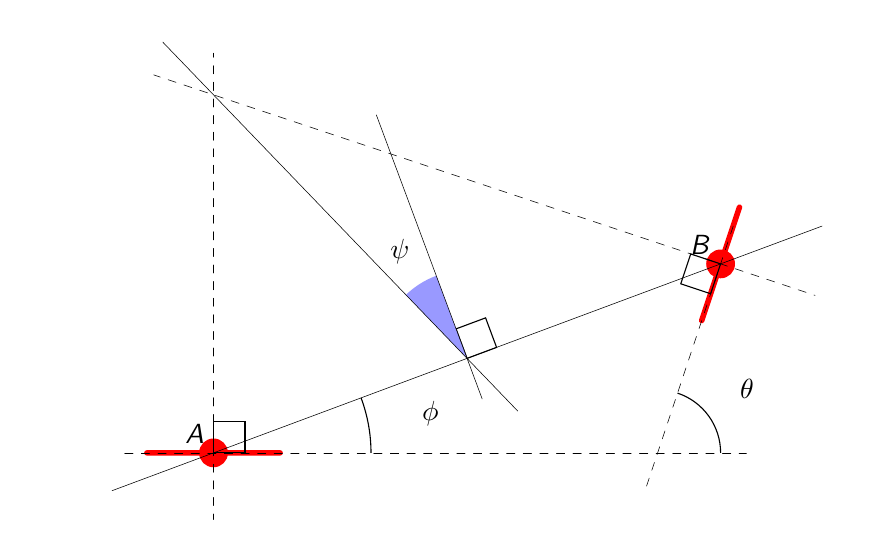
\begin{tikzpicture}[scale=.8, font=\sffamily]
% (C) edge schematics
  \begin{scope}[xshift=12.9cm, yshift=-8.5cm]
   \fill[white,fill opacity=.9] (0, 1.2) rectangle (13, 9);
%   \tkzInit[xmax=12, ymax=6]

    %----------------------------------------------------------
    % Defining coordinates
    %----------------------------------------------------------

   \tkzDefPoint(2.95, 2.25){A}
   \tkzDefPoint(11,5.25){B}
   \tkzLabelPoints[above left](B,A)
   \tkzDefPoint(10, 2.25){C}
  
   % draw red dots at the center of edges
   \tkzDrawPoints[size=10, color=red, fill=red](A,B)

    %----------------------------------------------------------
    % Drawing the lines and segments
    %----------------------------------------------------------
    \tkzDrawLine[color=red,line width=2pt, add=-1.15 and -.15 ](C,A)
    \tkzDrawLine[color=red,line width=2pt, add=-1.3 and -.3 ](C,B)
  
    \tkzDrawLine(A,B)
    \tkzDrawLines[dashed](A,C B,C)

   % drawing arcs for angles  
   \tkzMarkAngle[size=2.5,mkpos=.2](C,A,B)
   \tkzLabelAngle[pos=3.5,circle](C,A,B){$\mathsf{\phi}$}

   \tkzDefPointWith[linear,K=1.5](A,C)
   \tkzGetPoint{D}
   \tkzDefPointWith[linear,K=.75](B,C)
   \tkzGetPoint{E}
   \tkzMarkAngle[size=1,mkpos=.2](D,C,E)
   \tkzLabelAngle[pos=1.75,circle](D,C,E){$\mathsf{\theta}$}

    %----------------------------------------------------------
    % Drawing normals
    %----------------------------------------------------------

    \tkzDefLine[perpendicular=through A, K=-.75](C,A)
    \tkzGetPoint{a1}
    \tkzDefLine[perpendicular=through B, K=2.5](C,B)
    \tkzGetPoint{b1}
    \tkzInterLL(a1,A)(b1,B)  \tkzGetPoint{H}
    \tkzMarkRightAngle[size=.5](H,A,C)
    \tkzMarkRightAngle[size=.5](H,B,C)
    \tkzDrawLines[dashed,dash phase=1.5pt](a1,A)
    \tkzDrawLines[dashed,dash phase=0.5pt](b1,B)

    %----------------------------------------------------------
    % Drawing mediator and psi line
    %----------------------------------------------------------
%    \tkzDefLine[mediator](A,B)          \tkzGetPoints{m1}{M}
    \tkzDefMidPoint(A,B)
    \tkzGetPoint{M}
    \tkzDefLine[perpendicular=through M, K=.4](A,B)
    \tkzGetPoint{m1}
    \tkzMarkRightAngle[size=.5](B,M,m1)    
    
    \tkzFillAngle[size=1.4,fill=blue!40](m1,M,H)
    \tkzLabelAngle[pos=2,circle](m1,M,H){$\mathsf{\psi}$}%= \phi -\theta/2
    \tkzDrawLines[](m1,M M,H)
    
  \end{scope}
\end{tikzpicture}
} 
\vspace*{-5cm} 
\caption{ 
{\bf Measuring edge co-occurrences.} 
The relationship between a pair of edges can be quantified 
in terms of the difference between their orientations $\theta$, 
the ratio of scale $\sigma$ relative to the reference edge, 
the distance $d$ between their centers, 
and the difference of azimuth (angular location) $\phi$ 
of the second edge relative to the reference edge. 
Additionally, we define $\psi=\phi - \theta/2$ as it is
symmetric with respect to the choice of the reference edge, 
in particular, $\psi=0$ for co-circular edges.\label{fig:angles} %
 } %
\end{figure} %
%------------------------------%
%}
As in~\citet{Geisler01}, 
we will now measure the statistics of edge co-occurences 
using the definitions presented in main text Figure~1-B. 
We will be using the edges that we extracted 
following the method presented in the previous section. 
Note that since we are considering only relative orientations, 
co-occurrences have several geometrical symmetries: %.\ref{fig:angles}).: 
if an occurrence exists for a configuration $(\phi, \theta)$, then it exists also for 
$(\phi+\pi, \theta+\pi)$ (considering other orientations of the first edge by a rotation of $\pi$ radian),
$(\phi+\pi-\theta, \pi-\theta)$ (swapping both edges) and 
$(\phi-\theta, -\theta)$ (rotation of $\pi$ radians). 
For that reason, it is convenient to define $\psi=\phi - \theta/2$ (see main text Figure~1-B).
As $\psi$ is symmetric with respect to the choice of the reference
edge, for a configuration $(\psi, \theta)$, we have also the following
symmetries $(\psi+\pi, \theta+\pi)$, $(\psi+\pi, \pi-\theta)$ and
$(\psi, -\theta)$.

Geometrically, $\psi$ is the angle between 
(1) the mediator of the segment joining the edges' centers and 
(2) the line joining the center of this segment 
to the intersection of the normal of the segments (see  main text
Figure~1-B). %SI Figure~\ref{fig:angles}). 
Note that for a pair of edges on a common circle, 
we have $\phi=\theta/2$, that is, $\psi = 0$ (see the central vertical
axis in main text Figure~2).  This convention gives a simpler
representation of circularities (for similar approaches
see refs.~\autocite{Motoyoshi10,Sigman01,Hunt11}), and $\psi$ will denote
the difference of azimuth in the rest of the paper.  Colinearity
($\theta=\psi = 0$) and other parallel edges ($\theta = 0$)
are represented on the central horizontal axis of main text
Figure~2.

Main text Figure~2 shows a horizontal periodicity of $\pi$, a vertical
periodicity of $\pi$, and a mirror symmetry around the horizontal axis $\theta=0$. 
Furthermore, we observed that there is typically an axial symmetry 
with respect to the mediator
(that is, in any given image set, a configuration $(\psi, \theta)$ is
as likely as $(-\psi, \theta)$), corresponding to mirror versions of
images around the vertical axis $\psi=0$.
Due to the finite number of measurements, empirical results
(see SI Figure~\ref{fig:geisler}-A, or figure 3-C
from~\citet{Geisler01}) will of course not have perfect symmetry in practice.
Since $\phi$, $\psi$ and $\theta$ are angles defined 
for instance between $-\pi$ and $\pi$, these symmetries allows us to consider only a single quadrant 
(by convention the upper right, that is 
$-\pi/2 < \phi \leq \pi/2$,  $-\pi/2 < \psi \leq \pi/2$ and $0 \leq \theta \leq \pi/2$), 
the rest being inferred by the above relations. 
We used this additional looser type of symmetry only for simplifying
visualizations, not for the underlying calculations.

\subsection{Classification method}
\label{sec:SVM}
To validate the categorization performance, 
we used the standard SVM library as implemented by~\textcite{Pedregosa11}. 
First, we  randomly divided each database into a training and a testing sub-set.
In order to evaluate a distance between histograms, 
we used the Jensen--Shannon divergence distance
as a metric between histograms~\autocite{Cha02}. %, 
Thus, we directly supplied a precomputed Gram matrix of the distance 
between each pair of histograms to the classifier. 
We used the default parameters of the method. 
Other choices of parameters or of kernels 
(that is, between linear, radial basis functions, or precomputed) 
gave qualitatively similar results. 
Fitting the classifier to the training set was done using an 
automatic line search algorithm from the same library~\cite{Pedregosa11}.
The results of the SVM classifier are usually given as the precision, recall, or F1 score.
Here we used the latter  to directly compare our method to that of~\textcite{Serre07}.
This process was cross-validated 20 times 
by drawing new training and testing sets. 
Using these different trials,
we could measure the variability of the F1 score.
The variability was always in the range of $\approx 4\%$.
%%%%%%%%%%%%%%%%%%%%%%%%%%%%%%%%%%%%%%
\section{Supplementary Results: categorization using the statistics of edge co-occurrences}%
%%%%%%%%%%%%%%%%%%%%%%%%%%%%%%%%%%%%%%
Our goal is to study how the statistics of edge co-occurrence vary across three image categories, 
so we defined three testing databases. 
The first two consist of the image databases ($600$ images each)\footnote{Publicly available at {\it http://cbcl.mit.edu/software-datasets/serre/SerreOlivaPoggioPNAS07}.} used by~\textcite{Serre07}, 
which contain either animals at different close-up views in a natural setting (which we call ``animal image''), 
or natural images without animals, which we call ``non-animal natural images''. 
A third database for comparison consists of self-acquired images from a biology laboratory setting, 
containing $600$ indoor views of furniture, windows, and doors and cages in which animals are reared (which we call ``man-made images'').  

\subsection{First-order statistics}
%------------------------------------------------------------------------------------------------%#

One obvious candidate representation for categorization is the first-order statistics of edges. 
In natural images, edges are more frequently aligned to the cardinal axes, 
especially for man-made scenes, as has been reported and modeled previously by others~\autocite{Girshick11}. 
As the spectrum of edges is localized in the Fourier domain~\autocite{Fischer07cv}, 
the representation of first-order statistics of edges is equivalent 
to using the amplitude spectrum obtained by Fourier analysis of the raw image. 
The spectral signature of scenes has previously been used by computational models 
to infer scene categories~\autocite{Oliva01,Torralba03}), 
and the human visual system could take advantage of these low-level natural image statistics. 
To compare with these previous results, 
we computed first-order statistics on the sparse representation described in the methods section. 
The histograms yielded similar results to those found 
on the amplitude spectrum of the raw image~\autocite{Oliva01,Torralba03}.
However, these first-order statistics, 
while tending to be different on average for different scene categories, 
are also highly variable within each category. 
The first-order histogram is highly dependent on geometrical constraints 
that are independent of the scene category, 
like the field of view (close-up or full-field view) 
or the orientation relative to the horizon, 
and we show below that they are not particularly reliable for 
classifying individual images into these different categories (see Table in main text). 
Most importantly, these results fall to chance level with 
a rotation of the image or to changes in the spectral envelope, 
in contradiction with behavioral results~\autocite{Crouzet11b,Gaspar09}.
First-order statistics are therefore a relatively poor indicator of scene category. 

\subsection{Statistics of edge co-occurrences}
\label{sec:SO_res}
%------------------------------------------------------------------------------------------------%
Statistics of edge co-occurrences could represent a better alternative. 
Indeed, image semantics seem to depend not on spatial-frequency amplitude, 
but rather on phase information~\autocite{Oppenheim81}, 
which is also essential for discriminating textures~\autocite{Motoyoshi10}. 
Like~\textcite{Geisler01}, we have chosen to compute the histogram of edge co-occurrences, 
that is, the frequentist probability of an edge knowing a reference edge 
(yielding $N \cdot (N-1) /2=523776$ samples per image when using $N=1024$ edges as we do here). 
This histogram is a 4-dimensional function of 
(1) the distance $d$ between two edges,
(2) the difference of azimuth $\phi$ of the center of one edge with respect to
the position and orientation of the reference edge, 
(3) the difference of orientation $\theta$ between the two edges, and 
(4) the ratio of edge scales $\sigma$ (see diagram in  main text Figure~1-B). %SI Figure~\ref{fig:angles}). 
By definition of our representation, this set of statistics is independent 
of translations, rotations in the image plane, and scalings. 

First, we replicated the results of~\textcite{Geisler01} 
on a set of natural images to validate our procedure, 
from the edge representation to the extraction. 
We computed similar projections of the histograms as in~\textcite{Geisler01} and
found qualitatively similar results despite the different datasets and methods used. 
As in~\textcite{Geisler01}, the finding is that in natural images, edges are
more likely to be organized in co-linear or parallel textures (see SI Figure~\ref{fig:geisler}-A) 
and along co-circular paths with a prior for low curvatures (see SI Figure~\ref{fig:geisler}-B). 
What is more interesting is that when using images from different environments 
such as a man-made environment (brownish edges in the figure), 
one finds a different pattern, where co-linearity dominates.
This qualitative difference clearly indicates that the statistics of edge co-occurrences 
differ between databases. 
However, the precise way in which these sets differ is not necessarily clear, 
which will be analyzed in the next section. 

%: fig:geisler
\begin{figure}
\centering{%
% elephant:serre07_targets_B_N107001
%\pgfdeclareimage[interpolate=true,width=5cm,height=5cm]{image1}{../database/serre07_targets/B_N771063.jpg}
%\pgfdeclareimage[interpolate=true,width=5cm,height=5cm]{image1}{../database/serre07_distractors/Hda_obj252.jpg}
%$ cp ../figures/edges/classifier_serre07_distractors/Hda_obj252.jpg\[6\,\250\,\ 6\,\ 250\]_reconstruct.png figure1C.png
% TODO : use                 \node[anchor=north west, inner sep=0pt, outer sep=0pt] at (0,0) {\includegraphics[width=\imagewidth]{img/Haberthuer2010/R108C21Cb_s33358_normalize}};%
%\pgfdeclareimage[width=6.1cm,interpolate=false]{geisler}{figure1DE.pdf}
%%\pgfdeclareimage[width=6.1cm,interpolate=false]{geisler_colin}{figure1D.pdf}
%%\pgfdeclareimage[width=6.1cm,interpolate=false]{geisler_cocir}{figure1E.pdf}
\begin{tikzpicture}[scale=1, font=\sffamily]%,every node/.style={minimum size=1cm},on grid]

\node [anchor=south west] (SM2A) at (0, 4.25) {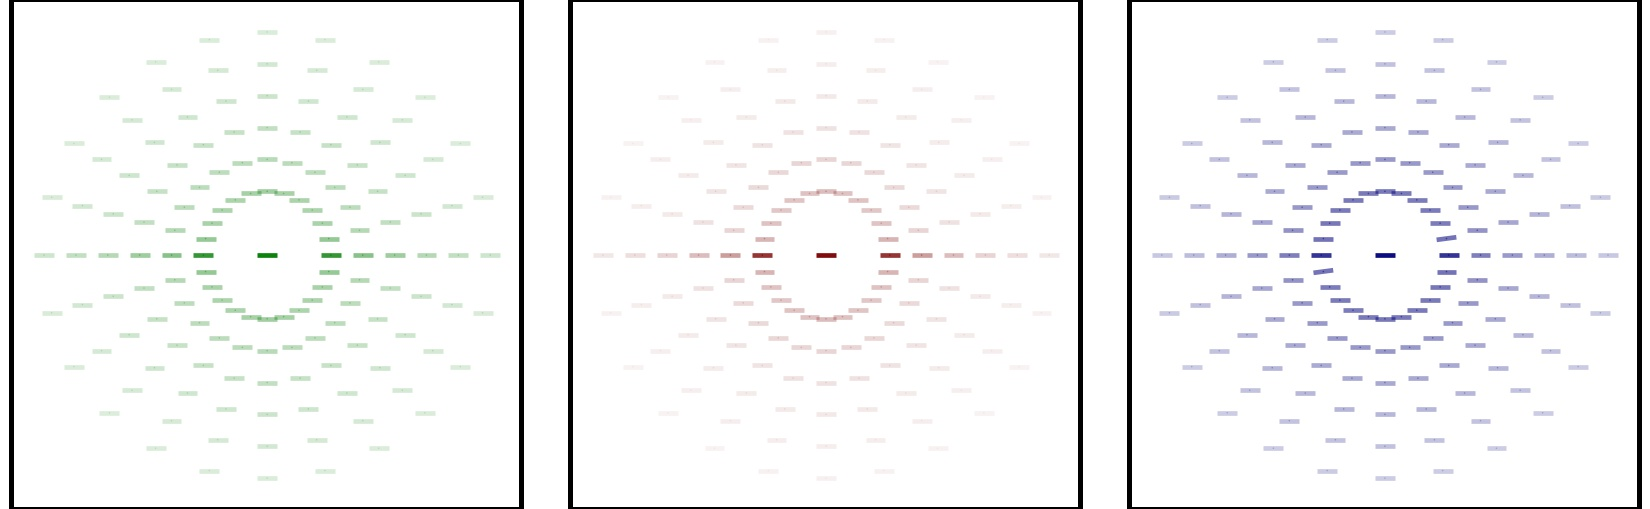
\includegraphics[width=.96\textwidth]{figureSM2A}};
\node [anchor=south west] (SM2B) at (0, 0.) {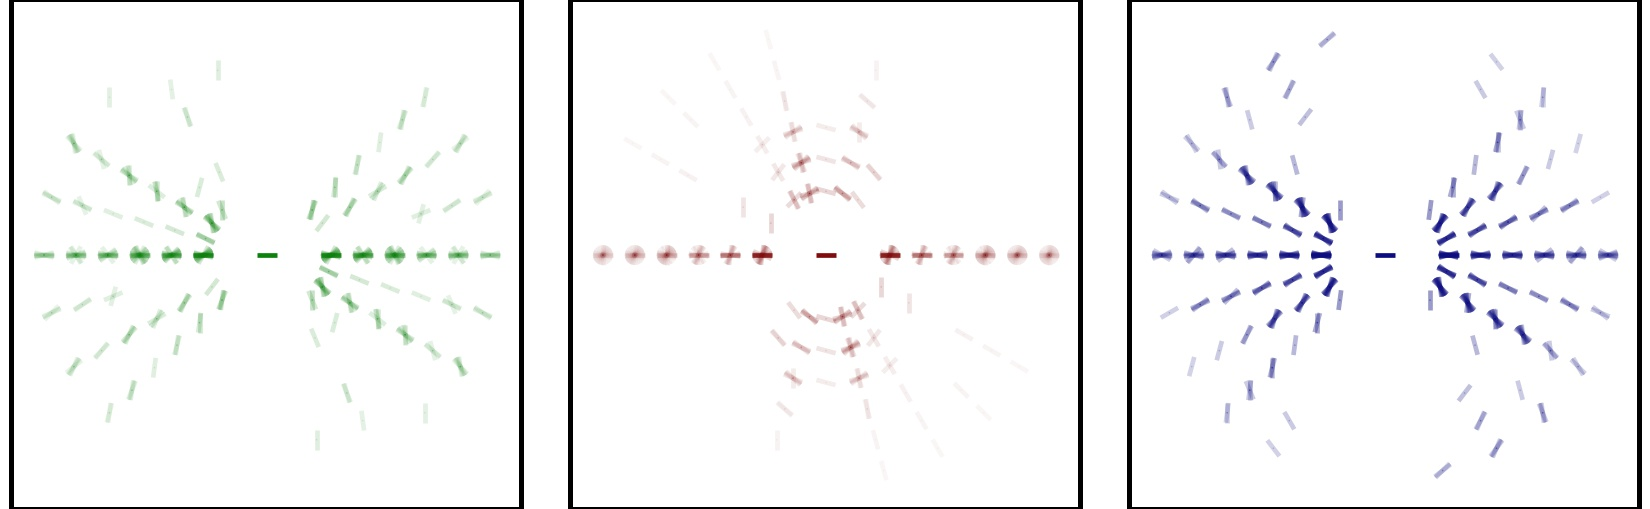
\includegraphics[width=.96\textwidth]{figureSM2B}};


\draw [anchor=south west] (0, 7.90) node {$\mathsf{(A)}$ Co-linearities~ $\arg\max_\theta p( \theta | d, \phi)$};
\draw [anchor=south west] (0, 3.65) node {$\mathsf{(B)}$ Co-circularities~$\arg\max_\phi p(\phi | d, \theta)$};

% vertical marker
\begin{scope}[xshift=-.225cm, yshift=.7465cm]
	\draw [thick,black!90] (2.235, 6.25) node[right]{} to (2.235, 6.5);
	\draw [black!90] (2.235, 6.375) node[right]{$\mathsf{\phi = \frac \pi 2}$};

	\draw [thick,black!90] (2.235, 4.25) node[right]{} to (2.235, 4.5);
	\draw [black!90] (2.235, 4.375) node[right]{$\mathsf{\phi = -\frac \pi 2}$};

	\draw[thick](3.1, 5.42) node[right]{} to (3.35, 5.42);
	\draw(3.225, 5.42) node[below]{$\mathsf{\phi = 0}$};
       
	\draw[thick](1.2, 5.42) node[right]{} to (1.45, 5.42);
	\draw(1.325, 5.42) node[below]{$\mathsf{\phi = \pi}$};
\end{scope}

\begin{scope}[xshift=5.93cm, yshift=5.05cm]
\draw[|<->|,thick,fill=black!90](0, 0)node[above]{} to (1.6, 0);
\draw(.8, 0)node[below]{$\mathsf{d = 1.23^o}$};
\end{scope}

\begin{scope}[xshift=0cm, yshift=-.30cm]
	\definecolor{greenish}{rgb}{0.05, 0.5, 0.05} % = natural
	\definecolor{brownish}{rgb}{0.5, 0.05, 0.05} % = man-made
	\definecolor{blueish}{rgb}{0.05, 0.05, 0.5} % = animal

    \draw[greenish, thick] (2.235, 0)node[above]{Non-animal};
    \draw[brownish, thick] (5.975, 0)node[above]{Man-made};
    \draw[blueish, thick] (9.735, 0) node[above]{Animal};
\end{scope}

\end{tikzpicture}
} 
%\vspace*{-.4cm} 
\caption{ 
{\bf Edge co-occurrences in different categories of natural scenes.} 
From the edge representation (see main text
Figure~1-A), it is possible to compute the statistics of edge
co-occurrences (see main text Figure~1-B) for each set of images.
Here we show a replication of the results from~\autocite{Geisler01}
for non-animal images (in greenish color), extended to man-made images
(in brownish color) and animals (in blueish color).
The statistics of edge co-occurrence correspond to a 4-dimensional histogram reporting, 
relative to a given edge, distance $d$, difference of azimuth $\phi$, difference of orientation $\theta$, and ratio of scale $\sigma$ as a single function $p(d, \phi, \theta, \sigma)$. 
$\mathsf{(A)}$~As in~\autocite{Geisler01}, we can project this function to see the most probable orientation difference 
knowing any possible position (determined by the distance $d$ and difference of azimuth $\phi$) 
relative to the reference edge (i.e., $\arg\max_\theta p( \theta | d, \phi)$). 
Note that we marginalize here relative to the scale $\sigma$, 
but that we observed that each individual scale behaved similarly, 
as expected by the invariance to zooms of these statistics. 
The results show that at every position, the most probable orientation of an edge 
is always parallel to the reference edge, 
reflecting a primary trend for parallel textures and patterns to occur in images of all categories.  
$\mathsf{(B)}$~Additionally, as in ref.~\autocite{Geisler01}, we can project this function 
onto other axes to show the most likely azimuth for 
each orientation difference and each given distance (i.e., $\arg\max_\phi p(\phi | d, \theta)$). 
The results show that when the difference of orientation $\theta$ is nonzero, 
it tends to be for co-circular contours (so-called ``good completions'') 
in natural images~\autocite{Sigman01} and in natural images containing an animal, 
while straight lines dominate in man-made images. 
Here, we have taken advantage of geometrical symmetries of edge co-occurrences 
to show only the top or the bottom of these configurations, respectively.
In both plots, the value of the maximum probability relative to the central reference edge 
is represented by the transparency of the edge shown and relative 
to the reference edge in the center of the plot. 
These results replicate ref.~\autocite{Geisler01} 
and suggest that statistics of edge co-occurrences in image categories
contain important information that could be used as a prior. 
In addition, while parallel textures dominate for all categories in $\mathsf{(A)}$, 
the pattern in $\mathsf{(B)}$ clearly differs qualitatively between databases, 
though further analysis in subsequent figures will be required 
to demonstrate these differences quantitatively.  
\label{fig:geisler} %
 } %
\end{figure} %
%------------------------------%

\subsection{Separating relevant variables in edge co-occurrences' statistics}
%------------------------------------------------------------------------------------------------%
The full set of second-order statistics is a function of four variables, 
which is difficult to plot and analyze, and so we considered 
whether it was possible to factorize this function into components that can be analyzed separately.  
We computed the mutual information of the joint probability 
with the $12$ possible combinations of the factorizations of $p(d, \phi, \theta, \sigma)$. 
This calculation gives different Kullback-Leibler distances~\autocite{Cha02} in bits 
between the factorizations and the original function, 
in order to measure the independence of each hypothesized factorization. 
For all sets of images, four good candidate factorizations emerge (see Table~\ref{tab:KL}): 
$p(\theta, \sigma, d)\cdot p(\phi)$, $p(\sigma, d, \phi)\cdot p(\theta)$, 
$p(\phi)\cdot p(\theta)\cdot p(\sigma, d)$ and $p(\phi, \theta)\cdot p(\sigma, d))$. 
An emergent pattern is that we may separate the characteristic angles 
($\phi$ and $\theta$, individually or together) 
from distance-related statistics ($d$ and $\sigma$). 
%Doing similar independence measures on $\psi$ and $\theta$ further showed 
%that these variables are relatively independent. 
%Thus, we can characterize images by two independent indices,
%one for collinearity, one for cocircularity. 
%To keep the generality of the results, we will in a first step study the whole $p(\psi,\theta)$ map. 
The distribution $p(d,\sigma)$ proved to be quite similar across the different classes of images, 
as it is more characteristic of the overall configuration of the scene 
than of the objects within it (see SI Figure~\ref{fig:chevrons}). 
% _____________________________________ %
\begin{table}[h!] 
\caption{{\bf Testing the relative dependence of all histogram variables.}
Given the histogram of second order statistics $p(d, \phi, \theta, \sigma)$ 
(which we will subsequently denote simply $p$), 
we have computed its entropy and the Kullback-Leibler (KL) divergence with all
combinations of the factorization of the variables $d$, $\phi$, $\theta$ and
$\sigma$ (in bits, averaged over all images from all categories). 
Entropy is the KL divergence of $p$ with the uniform distribution and serves as an upper bound.
The KL measure is positive and only the full statistics can achieve
$KL=0$ (by Gibbs' inequality), but the next four factorizations cause
very little error, and are thus good candidates. For these factorizations,
we may separate the characteristic angles ($\phi$ and $\theta$, individually or together) from
distance-related statistics ($d$ and $\sigma$) that are characteristic of the
configuration of the view. 
The remaining factorizations are much more different from the full distribution, 
and thus will not be considered further.\label{tab:KL}} 
\begin{center}
\begin{tabular}{@{\vrule height 1.5pt depth 4pt width 0pt}ll}
$Entropy(p)$ & $\approx 0.724$\\
 \hline \\[-1ex]
KL$(p || p)$ & $ = 0 $\\[1ex] 
KL$(p || p(\theta, \sigma, d)\cdot p(\phi))$               & $\approx  0.001$\\
KL$(p || p(\sigma, d, \phi)\cdot p(\theta))$               & $\approx  0.004$\\
KL$(p || p(\phi, \theta)\cdot p(\sigma, d))$               & $\approx  0.004$\\
KL$(p || p(\phi)\cdot p(\theta)\cdot p(\sigma, d))$        & $\approx  0.006$\\[1ex]
KL$(p || p(\phi, \theta, \sigma)\cdot p(d))$               & $\approx  0.057$\\
KL$(p || p(\theta, \sigma)\cdot p(d, \phi))$               & $\approx  0.058$\\
KL$(p || p(\theta, \sigma)\cdot p(d)\cdot p(\phi))$        & $\approx  0.058$\\
KL$(p || p(d, \phi, \theta)\cdot p(\sigma))$               & $\approx  0.059$\\
KL$(p || p(\sigma, \phi)\cdot p(d, \theta))$               & $\approx  0.060$\\
KL$(p || p(\phi, \theta)\cdot p(\sigma)\cdot p(d))$        & $\approx  0.060$\\
KL$(p || p(d, \phi)\cdot p(\theta)\cdot p(\sigma))$        & $\approx  0.061$\\
KL$(p || p(d)\cdot p(\phi)\cdot p(\theta)\cdot p(\sigma))$ & $\approx  0.061$
\end{tabular}
\end{center}
\end{table}
%------------------------------%

Let us now focus on the map of angle configurations 
$p(\phi, \theta)$: %\ref{fig:chevrons2}).  (see main text Figure~3)
This can be reduced to 2 dimensions, 
so that we can plot this probability as a ``chevron map'' $p(\psi, \theta)$.
Each chevron corresponds to a possible configuration of 
the angles $\psi = \phi - \theta/2$ and $\theta$. 
Such a map is shown in main text Figure~2 %\ref{fig:chevrons}-$\mathsf{C}$, 
with the saturation of the colored circle indicating the frequency of occurrence.
The chevron map spans each possible chevron configuration, 
i.e., for all possible difference of azimuth values $\psi$ on the horizontal axis 
and difference of orientation $\theta$ on the vertical axis. 
Red denotes more frequent than a uniform-probability reference, while
blue denotes less frequent. 

%------------------------------% 
%: fig:chevrons
\begin{figure}[!htb]
\centering{

}
\caption{ 
{\bf Configuration variables are not significantly different across categories.}  
An independence analysis shows that in natural images,
the statistics of edge co-occurrences can be factorized into 
independent components $p(\psi,\theta)\cdot p(\sigma,d)$ (see text). 
To show the shape of $p(\sigma,d)$, we plot in 
$\mathsf{(A)}$ the distribution of scale ratios $p(\sigma)$ and in 
$\mathsf{(B)}$ the distribution of distances to a reference edge $p(d)$. 
Counts are plotted for each dataset in the colors indicated 
(blue for non-animal, green for animals and red for man-made), 
along with the statistics obtained after shuffling each edge variable (in black). 
The bar heights allow comparison across categories, 
while the error bars indicate variation within each category. 
  We created a novel set by taking the extracted edges from the set of
  non-animal images, then shuffling the position of their centers
  ("shuffled set"), such that first-order information on orientation
  and scale is kept while all second-order statistical information
  (which relies on relative positions) is lost.
In $\mathsf{(A)}$ there is an overall decrease in probability 
with increasing difference in scale similar to that in the shuffled case, 
which is due to the finite number of scales. 
The distribution is consistent across all databases, 
with variability comparable within and  between databases, 
and thus the scale differences are not useful for categorizing the class of an image. 
%%%
Similarly, $\mathsf{(B)}$ shows that edges are relatively clustered, 
with other edges significantly more likely to be closer to a given reference edge 
(with a maximum of about $25\%$ more probable than in the shuffled case at the shortest range).
The results for shuffled images show that there is a bias due to the finite size of images. 
For non-shuffled images, the change in probability with distance is mainly due 
to a prior preference for a clustering of edges. 
This distribution is consistent with scenes consisting mostly of small objects, 
as is well described by the dead-leaves model~\autocite{Pitkow10}. 
Again, the variation within each database in $\mathsf{(B)}$ 
is high relative to the variation between them, and
so the distances are also not informative about the image class. 
\hide{
$\mathsf{(C)}$ 
A second component $p(\theta, \psi)$ 
represents the distribution of the different geometrical arrangements of edges' angles, 
which we call a ``chevron map'' (see main text Figure~2 and its description). 
For each chevron configuration, deeper and deeper red circles 
indicate configurations that are more and more likely 
with respect to an uniform prior (all configurations equally likely), 
with an average maximum of about $4$ times more likely, 
and deeper and deeper blue circles indicate configurations less likely 
than a flat prior (with a minimum of about $1.5$ times less likely). 
Conveniently, this ``chevron map'' shows in one graph (see  main text Figure~2)
that natural images 
have on average a preference for co-linear and parallel angles
(the horizontal middle axis, $\theta=0$), as seen in SI Figure~\ref{fig:geisler}-A, 
along with a slight preference for orthogonal configurations (top and bottom rows, $\theta \pm \pi/2$)).
Similarly, there are significantly more symmetric (that is collinear) configurations 
from the higher probability 
around the middle and border lines ($\psi =0$ or $\psi \pm \pi/2$),
as seen in SI Figure~\ref{fig:geisler}-B.
See main text Figure~3 %\ref{fig:chevrons2} 
to see that the chevron maps 
differ reliably between image classes, 
which will allow them to be used for classification.
}
\label{fig:chevrons}}% 
\end{figure}%
%------------------------------% 

%\showthe\columnwidth
Main text Figure~3 %\ref{fig:chevrons2} 
shows how the chevron map differs 
for the other two datasets, now relative to the map computed for the non-animal dataset. 
%Using the variability on an image-by-image basis, 
%we have plotted the $30\%$ most significantly different configurations in each map, 
%with respect to the estimated z scores for each chevron. 
A first observation is that main text Figure~3 %\ref{fig:chevrons2} 
shows the configuration in a more compact fashion than SI Figures~\ref{fig:geisler}-A and~\ref{fig:geisler}-B. 
In man-made versus natural non-animal environments, 
there is a significant excess of parallel and co-linear edges, 
with a maximum for the co-linear co-occurrence being about 2 times more likely than in natural non-animal images.
Interestingly, in animals versus non-animal scenes, 
there is a relative excess of co-circular and converging configurations, 
with a maximum being about 1.2 times more likely than in non-animal images. 
Note also a significant decrease for some configurations for man-made images 
than for other non-animal images (with a minimum being about 0.6 times less likely). 
This last point is consistent with the observation from ref.~\autocite{Hunt11}
that significant relationships may be either facilitating (for instance to group co-linear edges), 
or suppressive, to rule out some configurations as \textit{a priori} less probable.

In order to quantitatively assess the qualitative differences that we
observe in the chevron maps, we built a simple classifier to measure
if this representation is sufficient to categorize different image
categories.  Such a finding would suggest that information contained
in the statistics of edge co-occurrence in natural scenes may be used
instead of or alongside a hierarchical analysis of the visual scene,
when making a quick judgment as in rapid-categorization tasks.

%%%%%%%%%%%%%%%%%%%%%%%%%%%%%%%%%%%%%%
\subsection{Categorization of images using edge co-occurrences}

As described in the main text, 
we consider whether alternative low-level representations could be more
successful than the large set of such representations tested by~\textcite{Serre07}. 
For each individual image, we constructed a vector of features as either 
(FO) the histogram of first-order statistics, 
(SO) the full histogram of edge co-occurrences, or  
(CM) the histogram $p(\psi, \theta)$ corresponding to the chevron map. 
To compare the representational power of each type of feature vector, 
we gathered these vectors for each different class of images and 
tested a standard linear Support Vector Machine (SVM) classification algorithm, as described in Section~\ref{sec:SVM}. 
Our results can be compared directly to those of~\textcite{Serre07}, 
who used the same classifier on both the last level of their hierarchical representation (successfully), 
and directly on the raw images (unsuccessfully). 
They can also be compared with the other unsuccessful low-level representations 
tested by~\textcite{Serre07}, such as the mean luminance, a single-template SVM classifier, 
texton features, global (context) features, or the output of their model V1 complex cell layer.
%% see http://www.pnas.org/content/suppl/2007/03/23/0700622104.DC1/00622Table2.pdf
%% and http://cbcl.mit.edu/software-datasets/serre/SerreOlivaPoggioPNAS07/BenchmarkDB/index.html

As a control, we also used the nearest neighbor (that is, 2-means)
classifier. I.e., for any image, we computed the distance to the
average histogram (centroid) for each class.  Using a threshold, one
can decide which centroid is closer and classify the image to its
closest centroid. Averaged over all test images, this procedure gives
a quantitative measure of the compromise between correct hits and
false alarms with respect to the threshold; the measure is called the
Receiver Operating Characteristic (ROC). The final result is computed
as the Area Under the Curve (AUC). Globally, this method obtained
qualitatively similar results compared to the SVM algorithm. However,
the SVM algorithm performed slightly better in the vast majority of
cases.

Figure~4 in the main text gives the performance of different categorizations 
for the three types of representations, where several patterns can be seen. 
First, databases that are qualitatively different (such as non-animal versus man-made images) 
are very well categorized, with accuracy over 98\% when using the full statistics of edge co-occurrences. 
For images of man-made objects this result may be obvious, 
given their prevalence of highly regular co-linear edges. 
It is perhaps more surprising, particularly given the claims from~\textcite{Serre07} 
that low-level cues were unlikely to work, that we also achieved 
quite high, robust performance for classifying images containing animals versus other natural (non-animal) images.  
Second, it is interesting that results for the chevron map are almost as high 
as when using the full probabilities, 
confirming that the performance of the classifier comes primarily from a geometrical feature 
rather than a viewpoint-dependent feature (such as the scale of edges). 
This confirms our claim that configuration and geometrical variables are relatively independent 
(see SI Figure~\ref{fig:chevrons}).  
These results were also applied to a novel set of non-animal, animal and man-made images, giving similar results (see SI Figure~\ref{fig:SM_results}).

Our hypothesis is that classifying images containing animals versus
other natural non-animal images was successful because of the higher
prevalence of co-circular and converging contours in images containing
animals (see main text Figure~3). %\ref{fig:chevrons2}).
If humans are using similar mechanisms, their performance should
decrease with the size of the animal relative to its background,
because the statistics of the background will become more prominent.
Figure~\ref{fig:results-sub} shows that the model performance closely
tracks that of human observers on the image sub-categories defined
by~\textcite{Serre07} based on the closeness of the animals.
Performance for the first-order edge statistics does not similarly
vary, suggesting that they reflect incidental differences in the image
databases that are not due to the actual presence of the animal.
Performance for all the models is much higher on far images (where the
animal is very small) than for humans, presumably because the task did
not allow the humans to move their eyes during the presentation, and
the animals were not necessarily at the center of fixation.

% -------------------------------- %
%: fig:results
\begin{figure*}%[p]%[ht!]
\centering{
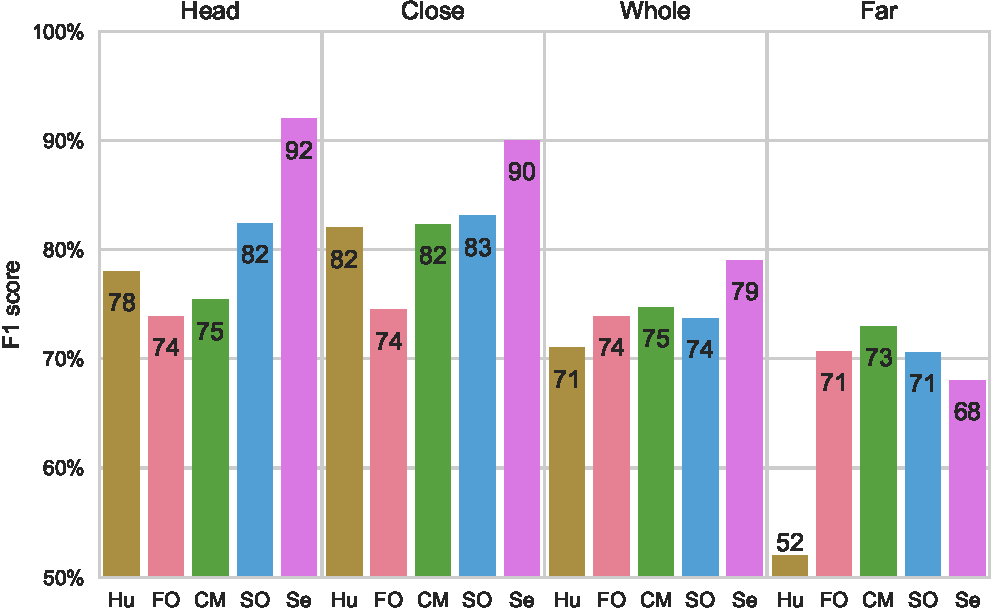
\includegraphics[width=\columnwidth]{figure_SM_subsets_results}%
}
\caption{%
Classification results (F1 score) within image subcategories, given for (Hu) human observers, (Se) the hierarchical model of~\textcite{Serre07}, and (FO, CM, and SO) the representations generated by our models.  Several patterns can be observed in these results. (1) Human performance falls to near chance level for detecting the `Far' animals, which is presumably because the relatively small animals in these images are not necessarily at the point of gaze, and in these experiments there is no time for making eye movements.  Conversely, all of the models outperform humans under these conditions, because they are provided the entire image.  (2) The FO model performance does not vary significantly with the size of the animal, suggesting that it is based on incidental features of the image datasets rather than the actual presence of an animal. (3) The CM and SO models track the patterns of performance for humans quite well, apart from the high performance for far images that all the models have.  (4) The Serre et al.\ model significantly outperforms humans in each category, which would be expected if it is modelling hierarchical processing strategies not available to humans in the rapid time scales of these experiments.
\label{fig:results-sub}}%
\end{figure*}%
% -------------------------------- %

% -------------------------------- %
%%%%%%%%%%%%%%%%%%%%%%%%%%%%%%%%%%%%%%%%%%%%%%%%%%%%%%%%%%%%
\subsection{Robustness to noise, translation and rotations}%
%%%%%%%%%%%%%%%%%%%%%%%%%%%%%%%%%%%%%%%%%%%%%%%%%%%%%%%%%%%%
Note that by definition, our measure of the statistics of edge co-occurrence 
is invariant to translations, scalings, and rotations in the plane of the image
(unlike the first-order statistics). 
Thus, despite any of these transformations, one can efficiently differentiate 
between images from different categories. 
This property makes it possible to explain the rather unintuitive result that
ultra-rapid categorization in humans is relatively independent to rotations~\autocite{Crouzet11b} 
(see also the supplementary information of~\textcite{Serre07}). 
We also performed the same classification where images from both databases 
were perturbed by adding independent Gaussian noise to each pixel 
such that signal-to-noise ratio was halved. 
As can be seen in Figure 4 of the main text and SI Figure 5, results are degraded but qualitatively similar. 
Edge extraction in the presence of noise may result in false edges, 
but the underlying statistics of the chevron maps are still robustly captured, 
thanks to the high number of co-occurrences that are measured.  

% -------------------------------- %
%: fig:results
\begin{figure*}%[p]%[ht!]
\centering{
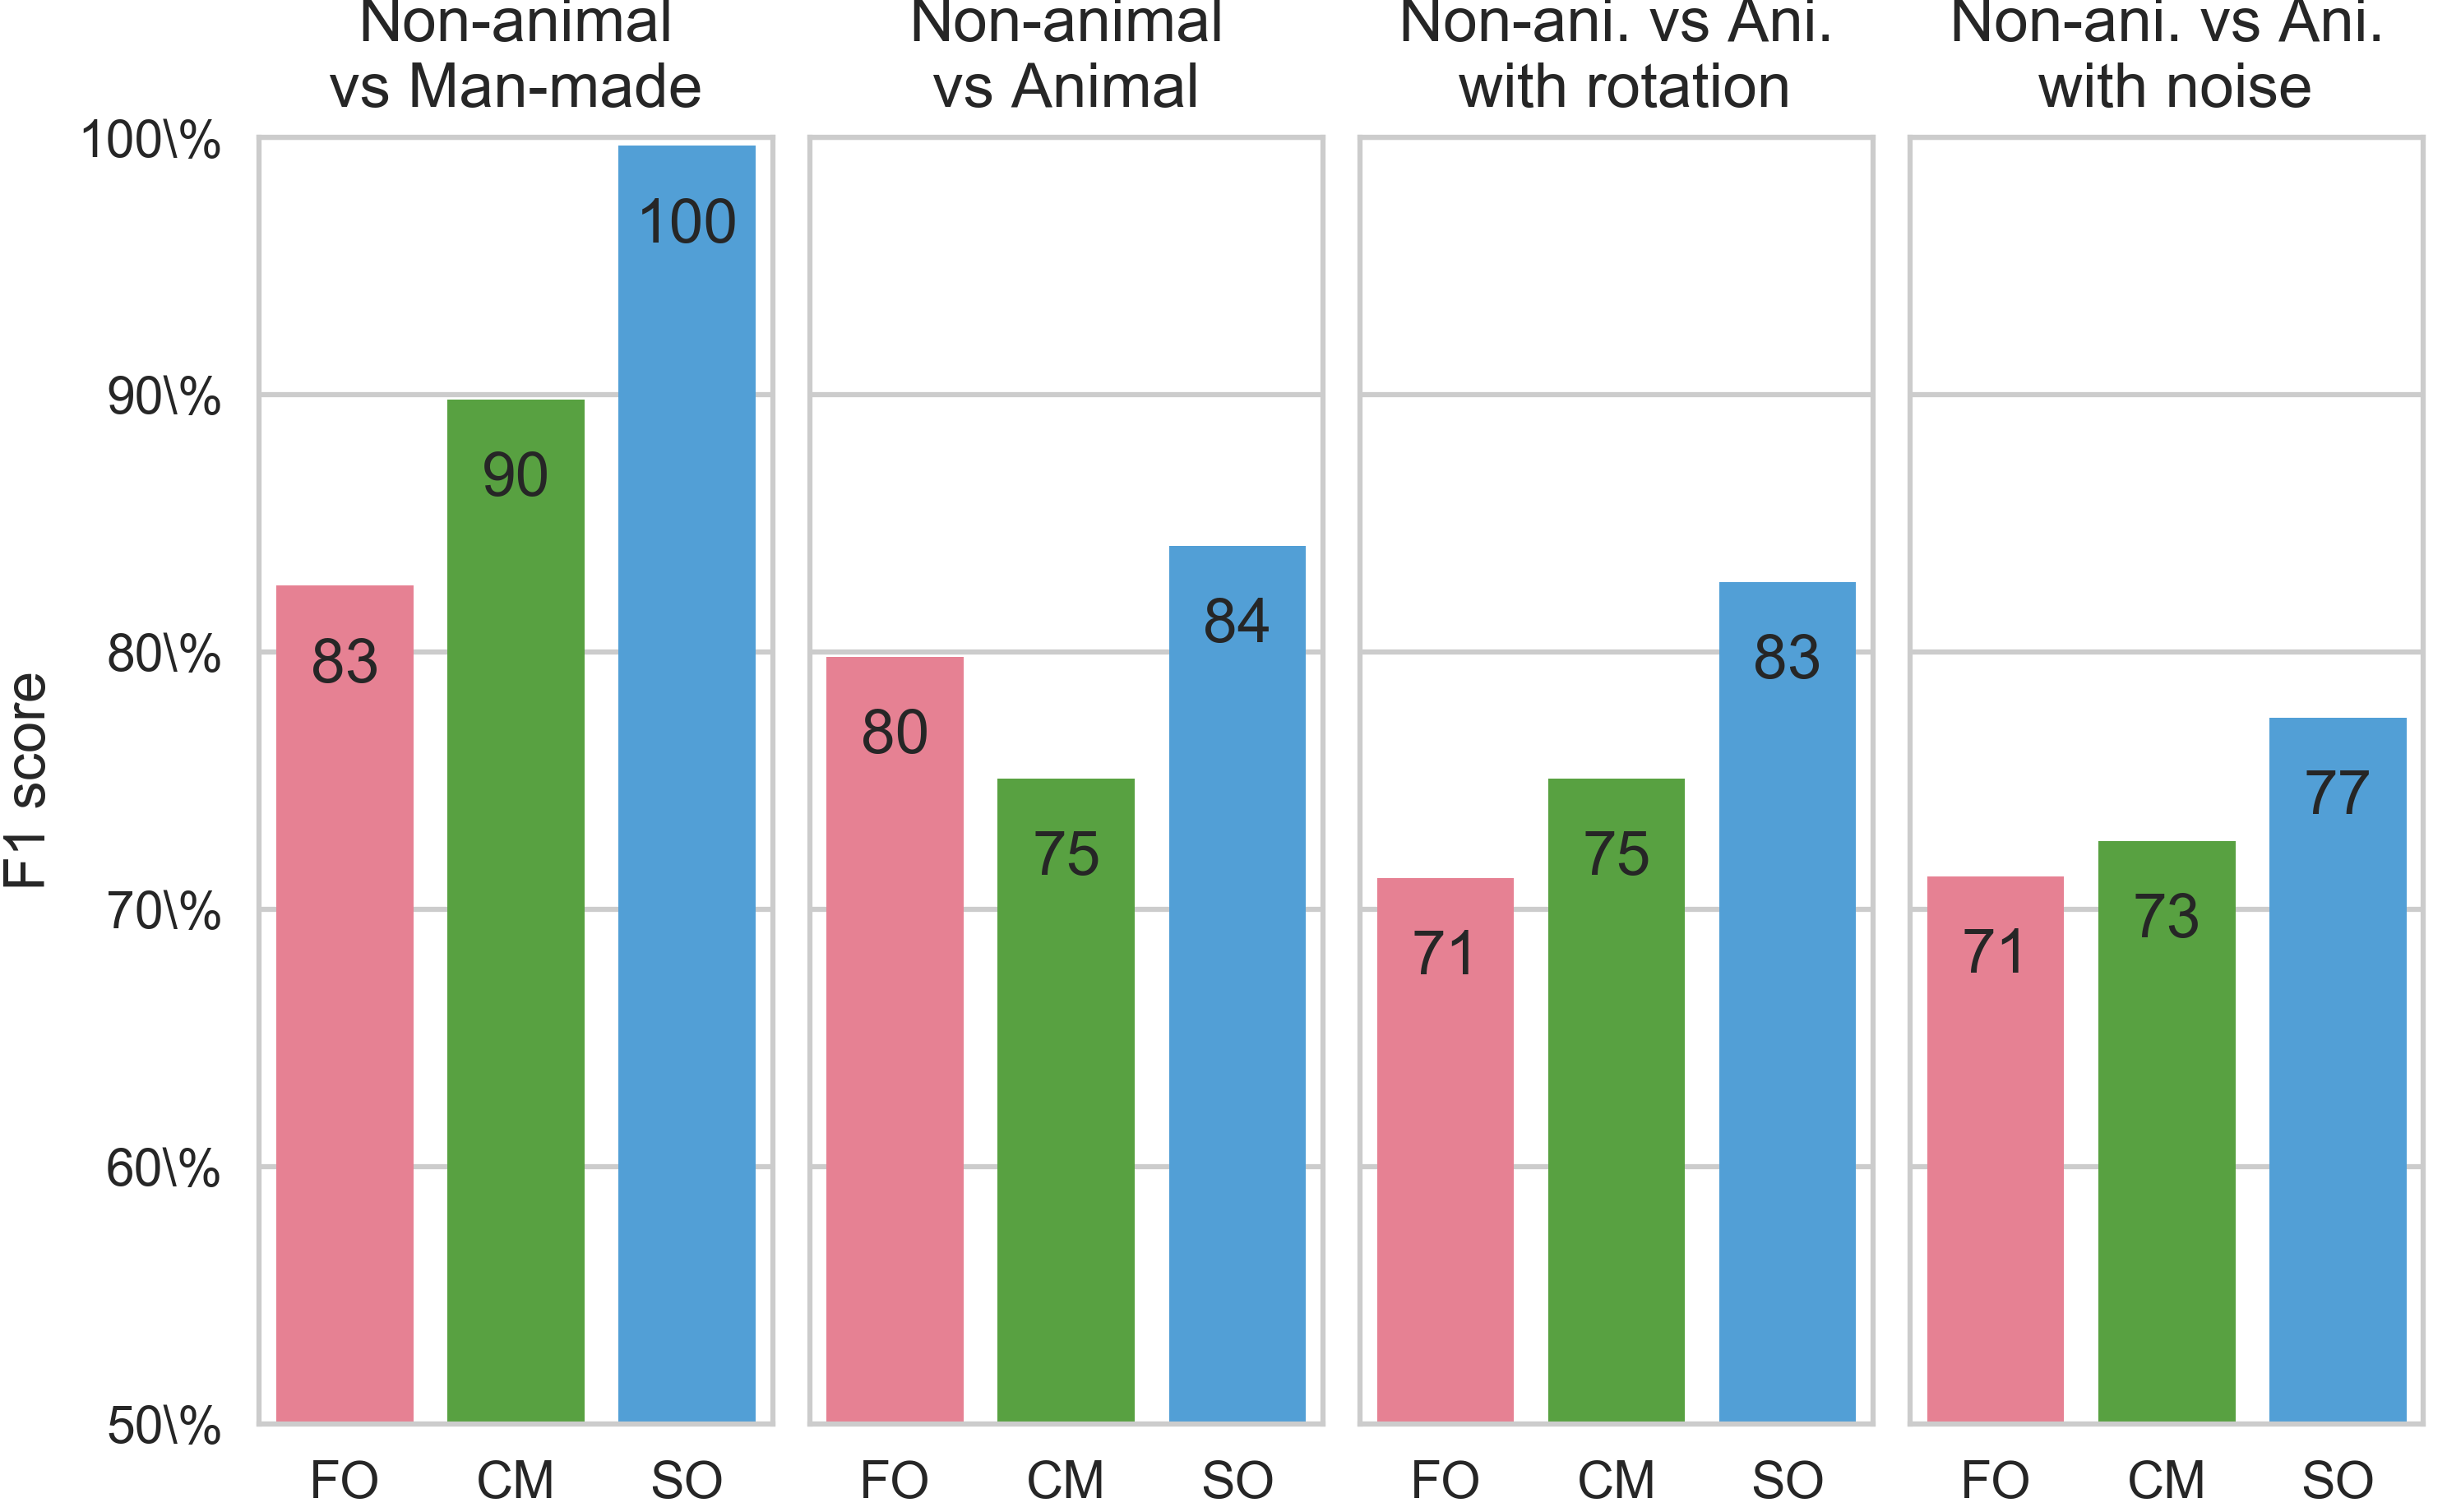
\includegraphics[width=\columnwidth]{figure_SM_results}%
}
\caption{%
Classification results on other datasets. 
To test the generality of the results presented in the main text, we applied the same method to additional collections of images from other sources.  These datasets were of similar size ($600$ images per database, each of size $244\times244$ pixels) as in the main text, but did not contain any of the same images as in the previous results. The non-animal and animal datasets originated from the same source as~\citep{Kirchner06,Crouzet10}, while the man-made dataset was a series of images taken in a different laboratory environment, from a previous study~\citep{Rudiger14cosyne}.
As for figure 4 of the main text, for each individual image, we constructed a vector of features as either 
%
(FO) the histogram of first-order edge statistics,
(CM) the two-dimensional chevron map subset of the second-order statistics (see Figure~\ref{fig:chevrons}), or
(SO) the full, four-dimensional second-order statistics.
%
  We gathered these vectors for each different class of images and
  report here the results of the SVM classifier using an
  F1 score (where 50\% represents chance level). Results are similar to those presented in the main text, except that for these datasets the animals are well categorized (F1 score$=78\%$) using first-order statistics alone. This appears to be due to a bias in that database's selection of non-animal images, which include wide landscapes and man-made scenes with easily detectable cardinal orientations. However, the first-order classification results decrease when a random rotation has been applied to the image (F1 score$=72\%$), while second-order features are insensitive to such perturbation (as for humans~\autocite{Crouzet11b}) and nearly insensitive to added noise, and thus they are a reliable indicator of image category.
\label{fig:SM_results}}%
\end{figure*}%
% -------------------------------- %
%\hide{%
%%%%%%%%%%%%%%%%%%%%%%%%%%%%%%%%%%%%%%
\section{Discussion}
%%%%%%%%%%%%%%%%%%%%%%%%%%%%%%%%%%%%%%
%%%%%%%%%%%%%%%%%%%%%%%%%%%%%%%%%%%%%%
Using standard tools from different disciplines 
(image processing, machine learning, neuroscience), 
we have provided a novel categorization algorithm that
has potential impact on all three fields. 
Our main results are that statistics of edge co-occurrence 
can be computed reliably for natural images, 
and that they contain important information about local geometry 
that is sufficient to categorize individual images accurately. 
These results call into question previous claims that a hierarchical, 
semantic-like, analysis of the visual scene is necessary 
for classification into high-level categories~\autocite{Serre07}. 

We speculate that the observed differences in second-order statistics for images
with animals have an underlying basis in the physical constraints 
governing the shapes of animals, compared to other natural stimuli. 
Specifically, animals generally have compact shapes, constrained by their capacity to move, 
unlike plants, for instance, which are rooted in one location 
and often become elongated as they stretch to reach towards sunlight. 
The bodies of animals are also often enveloped by a flexible membrane, 
which by the constraint of minimal surface area will tend to assume a circular shape, 
just as a bubble will. 
These overall principles for shape patterning are echoed in subparts of the body, 
such as the eyes and the hair, markings, and textures that pattern the skin of the animal, 
further biasing the statistics. 
Conversely, man-made objects tend to have long, straight lines, 
with sharp orthogonal edges due to their methods of manufacture. 
We would expect that other categories of objects could similarly be
distinguished by their second-order statistics, 
assuming that their form %of those objects 
follows their function in ways analogous to the categories tested
here.  Thus we expect that the second-order statistics will be useful
as a general method for distinguishing a wide range of scene and
object categories.

Several improvements to the method could be considered for future applications.
First, the image processing methods that are used to represent the data that is
used to reach a classification result can be extended. 
For instance, edge extraction algorithms are mostly based 
on measuring a match between the raw image and a model of an edge (a log-Gabor patch, in this case). 
Using the average prior on edge co-occurrences 
(knowing their distance as in SI Figure~\ref{fig:chevrons}-B 
or edge configuration as in SI Figure~\ref{fig:chevrons}-C), 
corresponding to average knowledge across all image classes (the so-called ``association field''), 
one could improve the measure of this match by accumulating knowledge from neighboring edges, 
thus improving the overall signal-to-noise ratio. 
Moreover, using the prior knowledge that this image belongs to a certain class 
(for instance due to some contextual cue), 
this match can be improved by using the expected second-order statistics 
for that class as a prior probability. 
Results from monkey primary visual cortex suggest that animals may similarly 
be able to modulate their association field dynamically.  
For instance, \textcite{McManus11} reported a gating of horizontal connections 
dependent on the task (detecting collinear or cocircular edges), 
which is similar to what we show in main text Figure~3 %\ref{fig:chevrons2} 
if we assume that these tasks correspond 
to the categorization of natural images versus man-made or animal images. 
Finally, these algorithms can also be complemented with a segmentation scheme 
using a local classification rule similar to the one we proposed here. 
Images containing animals usually consist of a figure (the animal), 
and a background consisting of a natural image without an animal. 
Classifying the category of each edge using such a method 
would itself allow refining the histogram for each class and the
corresponding chevron maps, along with providing a segmentation of each image.
Ultimately, such a method should help to improve the measurement of edge
co-occurrences and the different patterns associated with different classes of objects.

% ??? does this explain recognition in Brady08?
We predict that this result can be used to improve existing machine learning algorithms 
for visual scene comprehension. 
Despite the intensive focus in the machine-learning community 
on improving algorithms for classifying images, 
to our knowledge the second-order statistics have not previously been tested as a representation. 
In contrast, hierarchical models such as deep-learning networks 
have recently attracted a great deal of attention, 
in part due to their presumed similarity with the architecture of the cortex. 
The dependence between variables within one level of the architecture is often overlooked, 
assuming that it would lead to intractable algorithms. 
Here, we focused on the statistics of edge co-occurrences 
and used a classical classification method (SVM) as a generic illustration for its performance. 
The objective was to prove the usefulness of such a simple, one-layer representation. 
Ultimately, this approach could be integrated with more complex models 
such as the one proposed by~\textcite{Serre07}. 
The probabilistic setting common to such models would allow a seamless integration 
that has already been proven efficient for predicting biological results~\autocite{Rao99,Lee03}. 

Finally, these results are highly relevant for neuroscience.
First, they challenge the premise that ten ``processing layers'' 
are necessary to categorize image classes, 
a premise that is the root of the hypothesis that ultra-rapid categorization 
necessarily implies that only a few spikes per neuron are used~\autocite{Thorpe01}. 
Instead, they suggest a complementary source of information based on the computation of 
the probability of co-occurrences using intra-cortical connectivity (lateral connections). 
As such, we offer a simple explanation of the role of lateral interactions 
in lower visual areas~\autocite{Bosking97,Hunt11}. 
This source of information would be integrated at the same time 
as the feed-forward pass and would share some of the same mechanisms, 
such that they would lead to a progressive refinement of the representation of information. 
We propose that the statistics of edge co-occurrences play an important role 
in the performance measured in experiments measuring ultra-rapid categorization. 
% If the images that are miscategorized by humans have 2nd-order statistics that
% are more similar to the opposite database, that would be strong%% support for
% our hypothesis..
%It should be noted that predictive coding in the cortex remains a controversial
%hypothesis. Some of its controversy stems from findings that sometimes a match
%between sensory signals and descending predictions leads to the enhancement of
%neuronal firing, and not its cancellation~\autocite{Wannig11}. 
A further prediction would be that that categorization 
could be manipulated by modifying edge co-occurrence in a set of images 
(e.g., producing an image containing animals but with the statistics of the 'natural' set, and vice versa); 
rapid human responses are predicted to primarily follow the statistics of edge co-occurrences, 
rather than the actual presence of an animal. 
I.e., this approach predicts that an image with significantly more curves than a typical image 
would be falsely detected to contain an animal, in a rapid categorization task. 

Second, these results have consequences for our interpretation of the observed pattern 
of lateral interactions in V1, such as the results of~\textcite{Bosking97},
and therefore on our understanding through models~\autocite{Garrigues08,Bednar12jpp}. 
If the lateral connection patterns are learned by experience-driven plasticity~\autocite{Callaway90}, 
we predict that the patterns in wild-raised tree shrews would be very different 
from those measured by~\textcite{Bosking97} and analyzed by~\textcite{Hunt11}, 
with shorter-range correlations and less emphasis on co-linear continuations. 
This prediction can be tested in future experiments on matching groups 
of animals reared in different environments. 
From our results, we predict that $p(\theta, \psi)$ should be dynamically adaptive~\autocite{McManus11}, 
since it varies strongly across environments, while $p(d,\sigma)$ could safely be hard-wired. 
The biggest challenge is to understand how such probabilities 
may be represented in the neural activity and how the probabilistic calculations 
could be implemented in animal brains. 
%In particular, novel analysis of the data from~\textcite{Bosking97}
%by~\textcite{Hunt11} has suggested that co-circularity is weak but present, and
%also (surprisingly) that anti-cocircular edge co-occurrences may be connected.
%Indeed, an anti-circular arrangement is less-likely that normal, and therefore
%carries surprising information with respect to the model of smooth contours,
%possibly about contour disruption or the presence of corners. This confirms the
%idea of the brain as a generic information processing machine, but questions
%the actual information representation that may actually be used in the neural
%activity. %
%}%
\printbibliography
\end{document}%
